
%% bare_conf.tex
%% V1.4b
%% 2015/08/26
%% by Michael Shell
%% See:
%% http://www.michaelshell.org/
%% for current contact information.
%%
%% This is a skeleton file demonstrating the use of IEEEtran.cls
%% (requires IEEEtran.cls version 1.8b or later) with an IEEE
%% conference paper.
%%
%% Support sites:
%% http://www.michaelshell.org/tex/ieeetran/
%% http://www.ctan.org/pkg/ieeetran
%% and
%% http://www.ieee.org/

%%*************************************************************************
%% Legal Notice:
%% This code is offered as-is without any warranty either expressed or
%% implied; without even the implied warranty of MERCHANTABILITY or
%% FITNESS FOR A PARTICULAR PURPOSE! 
%% User assumes all risk.
%% In no event shall the IEEE or any contributor to this code be liable for
%% any damages or losses, including, but not limited to, incidental,
%% consequential, or any other damages, resulting from the use or misuse
%% of any information contained here.
%%
%% All comments are the opinions of their respective authors and are not
%% necessarily endorsed by the IEEE.
%%
%% This work is distributed under the LaTeX Project Public License (LPPL)
%% ( http://www.latex-project.org/ ) version 1.3, and may be freely used,
%% distributed and modified. A copy of the LPPL, version 1.3, is included
%% in the base LaTeX documentation of all distributions of LaTeX released
%% 2003/12/01 or later.
%% Retain all contribution notices and credits.
%% ** Modified files should be clearly indicated as such, including  **
%% ** renaming them and changing author support contact information. **
%%*************************************************************************


% *** Authors should verify (and, if needed, correct) their LaTeX system  ***
% *** with the testflow diagnostic prior to trusting their LaTeX platform ***
% *** with production work. The IEEE's font choices and paper sizes can   ***
% *** trigger bugs that do not appear when using other class files.       ***                          ***
% The testflow support page is at:
% http://www.michaelshell.org/tex/testflow/



\documentclass[conference]{IEEEtran}
% Some Computer Society conferences also require the compsoc mode option,
% but others use the standard conference format.
%
% If IEEEtran.cls has not been installed into the LaTeX system files,
% manually specify the path to it like:
% \documentclass[conference]{../sty/IEEEtran}





% Some very useful LaTeX packages include:
% (uncomment the ones you want to load)


% *** MISC UTILITY PACKAGES ***
%
%\usepackage{ifpdf}
% Heiko Oberdiek's ifpdf.sty is very useful if you need conditional
% compilation based on whether the output is pdf or dvi.
% usage:
% \ifpdf
%   % pdf code
% \else
%   % dvi code
% \fi
% The latest version of ifpdf.sty can be obtained from:
% http://www.ctan.org/pkg/ifpdf
% Also, note that IEEEtran.cls V1.7 and later provides a builtin
% \ifCLASSINFOpdf conditional that works the same way.
% When switching from latex to pdflatex and vice-versa, the compiler may
% have to be run twice to clear warning/error messages.






% *** CITATION PACKAGES ***
%
%\usepackage{cite}
% cite.sty was written by Donald Arseneau
% V1.6 and later of IEEEtran pre-defines the format of the cite.sty package
% \cite{} output to follow that of the IEEE. Loading the cite package will
% result in citation numbers being automatically sorted and properly
% "compressed/ranged". e.g., [1], [9], [2], [7], [5], [6] without using
% cite.sty will become [1], [2], [5]--[7], [9] using cite.sty. cite.sty's
% \cite will automatically add leading space, if needed. Use cite.sty's
% noadjust option (cite.sty V3.8 and later) if you want to turn this off
% such as if a citation ever needs to be enclosed in parenthesis.
% cite.sty is already installed on most LaTeX systems. Be sure and use
% version 5.0 (2009-03-20) and later if using hyperref.sty.
% The latest version can be obtained at:
% http://www.ctan.org/pkg/cite
% The documentation is contained in the cite.sty file itself.






% *** GRAPHICS RELATED PACKAGES ***
%
\ifCLASSINFOpdf
  % \usepackage[pdftex]{graphicx}
  % declare the path(s) where your graphic files are
  % \graphicspath{{../pdf/}{../jpeg/}}
  % and their extensions so you won't have to specify these with
  % every instance of \includegraphics
  % \DeclareGraphicsExtensions{.pdf,.jpeg,.png}
\else
  % or other class option (dvipsone, dvipdf, if not using dvips). graphicx
  % will default to the driver specified in the system graphics.cfg if no
  % driver is specified.
  % \usepackage[dvips]{graphicx}
  % declare the path(s) where your graphic files are
  % \graphicspath{{../eps/}}
  % and their extensions so you won't have to specify these with
  % every instance of \includegraphics
  % \DeclareGraphicsExtensions{.eps}
\fi
% graphicx was written by David Carlisle and Sebastian Rahtz. It is
% required if you want graphics, photos, etc. graphicx.sty is already
% installed on most LaTeX systems. The latest version and documentation
% can be obtained at: 
% http://www.ctan.org/pkg/graphicx
% Another good source of documentation is "Using Imported Graphics in
% LaTeX2e" by Keith Reckdahl which can be found at:
% http://www.ctan.org/pkg/epslatex
%
% latex, and pdflatex in dvi mode, support graphics in encapsulated
% postscript (.eps) format. pdflatex in pdf mode supports graphics
% in .pdf, .jpeg, .png and .mps (metapost) formats. Users should ensure
% that all non-photo figures use a vector format (.eps, .pdf, .mps) and
% not a bitmapped formats (.jpeg, .png). The IEEE frowns on bitmapped formats
% which can result in "jaggedy"/blurry rendering of lines and letters as
% well as large increases in file sizes.
%
% You can find documentation about the pdfTeX application at:
% http://www.tug.org/applications/pdftex





% *** MATH PACKAGES ***
%
%\usepackage{amsmath}
% A popular package from the American Mathematical Society that provides
% many useful and powerful commands for dealing with mathematics.
%
% Note that the amsmath package sets \interdisplaylinepenalty to 10000
% thus preventing page breaks from occurring within multiline equations. Use:
%\interdisplaylinepenalty=2500
% after loading amsmath to restore such page breaks as IEEEtran.cls normally
% does. amsmath.sty is already installed on most LaTeX systems. The latest
% version and documentation can be obtained at:
% http://www.ctan.org/pkg/amsmath





% *** SPECIALIZED LIST PACKAGES ***
%
%\usepackage{algorithmic}
% algorithmic.sty was written by Peter Williams and Rogerio Brito.
% This package provides an algorithmic environment fo describing algorithms.
% You can use the algorithmic environment in-text or within a figure
% environment to provide for a floating algorithm. Do NOT use the algorithm
% floating environment provided by algorithm.sty (by the same authors) or
% algorithm2e.sty (by Christophe Fiorio) as the IEEE does not use dedicated
% algorithm float types and packages that provide these will not provide
% correct IEEE style captions. The latest version and documentation of
% algorithmic.sty can be obtained at:
% http://www.ctan.org/pkg/algorithms
% Also of interest may be the (relatively newer and more customizable)
% algorithmicx.sty package by Szasz Janos:
% http://www.ctan.org/pkg/algorithmicx




% *** ALIGNMENT PACKAGES ***
%
%\usepackage{array}
% Frank Mittelbach's and David Carlisle's array.sty patches and improves
% the standard LaTeX2e array and tabular environments to provide better
% appearance and additional user controls. As the default LaTeX2e table
% generation code is lacking to the point of almost being broken with
% respect to the quality of the end results, all users are strongly
% advised to use an enhanced (at the very least that provided by array.sty)
% set of table tools. array.sty is already installed on most systems. The
% latest version and documentation can be obtained at:
% http://www.ctan.org/pkg/array


% IEEEtran contains the IEEEeqnarray family of commands that can be used to
% generate multiline equations as well as matrices, tables, etc., of high
% quality.




% *** SUBFIGURE PACKAGES ***
%\ifCLASSOPTIONcompsoc
%  \usepackage[caption=false,font=normalsize,labelfont=sf,textfont=sf]{subfig}
%\else
%  \usepackage[caption=false,font=footnotesize]{subfig}
%\fi
% subfig.sty, written by Steven Douglas Cochran, is the modern replacement
% for subfigure.sty, the latter of which is no longer maintained and is
% incompatible with some LaTeX packages including fixltx2e. However,
% subfig.sty requires and automatically loads Axel Sommerfeldt's caption.sty
% which will override IEEEtran.cls' handling of captions and this will result
% in non-IEEE style figure/table captions. To prevent this problem, be sure
% and invoke subfig.sty's "caption=false" package option (available since
% subfig.sty version 1.3, 2005/06/28) as this is will preserve IEEEtran.cls
% handling of captions.
% Note that the Computer Society format requires a larger sans serif font
% than the serif footnote size font used in traditional IEEE formatting
% and thus the need to invoke different subfig.sty package options depending
% on whether compsoc mode has been enabled.
%
% The latest version and documentation of subfig.sty can be obtained at:
% http://www.ctan.org/pkg/subfig




% *** FLOAT PACKAGES ***
%
%\usepackage{fixltx2e}
% fixltx2e, the successor to the earlier fix2col.sty, was written by
% Frank Mittelbach and David Carlisle. This package corrects a few problems
% in the LaTeX2e kernel, the most notable of which is that in current
% LaTeX2e releases, the ordering of single and double column floats is not
% guaranteed to be preserved. Thus, an unpatched LaTeX2e can allow a
% single column figure to be placed prior to an earlier double column
% figure.
% Be aware that LaTeX2e kernels dated 2015 and later have fixltx2e.sty's
% corrections already built into the system in which case a warning will
% be issued if an attempt is made to load fixltx2e.sty as it is no longer
% needed.
% The latest version and documentation can be found at:
% http://www.ctan.org/pkg/fixltx2e


%\usepackage{stfloats}
% stfloats.sty was written by Sigitas Tolusis. This package gives LaTeX2e
% the ability to do double column floats at the bottom of the page as well
% as the top. (e.g., "\begin{figure*}[!b]" is not normally possible in
% LaTeX2e). It also provides a command:
%\fnbelowfloat
% to enable the placement of footnotes below bottom floats (the standard
% LaTeX2e kernel puts them above bottom floats). This is an invasive package
% which rewrites many portions of the LaTeX2e float routines. It may not work
% with other packages that modify the LaTeX2e float routines. The latest
% version and documentation can be obtained at:
% http://www.ctan.org/pkg/stfloats
% Do not use the stfloats baselinefloat ability as the IEEE does not allow
% \baselineskip to stretch. Authors submitting work to the IEEE should note
% that the IEEE rarely uses double column equations and that authors should try
% to avoid such use. Do not be tempted to use the cuted.sty or midfloat.sty
% packages (also by Sigitas Tolusis) as the IEEE does not format its papers in
% such ways.
% Do not attempt to use stfloats with fixltx2e as they are incompatible.
% Instead, use Morten Hogholm'a dblfloatfix which combines the features
% of both fixltx2e and stfloats:
%
% \usepackage{dblfloatfix}
% The latest version can be found at:
% http://www.ctan.org/pkg/dblfloatfix




% *** PDF, URL AND HYPERLINK PACKAGES ***
%
%\usepackage{url}
% url.sty was written by Donald Arseneau. It provides better support for
% handling and breaking URLs. url.sty is already installed on most LaTeX
% systems. The latest version and documentation can be obtained at:
% http://www.ctan.org/pkg/url
% Basically, \url{my_url_here}.




% *** Do not adjust lengths that control margins, column widths, etc. ***
% *** Do not use packages that alter fonts (such as pslatex).         ***
% There should be no need to do such things with IEEEtran.cls V1.6 and later.
% (Unless specifically asked to do so by the journal or conference you plan
% to submit to, of course. )


% correct bad hyphenation here
\hyphenation{op-tical net-works semi-conduc-tor}
\usepackage{cite}
\usepackage{amsmath,amssymb,amsfonts}
\usepackage{subfigure}
\usepackage{algorithmic}
\usepackage{graphicx}
\usepackage{textcomp}
\usepackage{enumerate}
\usepackage{xcolor}

\begin{document}
%
% paper title
% Titles are generally capitalized except for words such as a, an, and, as,
% at, but, by, for, in, nor, of, on, or, the, to and up, which are usually
% not capitalized unless they are the first or last word of the title.
% Linebreaks \\ can be used within to get better formatting as desired.
% Do not put math or special symbols in the title.
\title{Bare Demo of IEEEtran.cls\\ for IEEE Conferences}


% author names and affiliations
% use a multiple column layout for up to three different
% affiliations
\author{\IEEEauthorblockN{Michael Shell}
\IEEEauthorblockA{School of Electrical and\\Computer Engineering\\
Georgia Institute of Technology\\
Atlanta, Georgia 30332--0250\\
Email: http://www.michaelshell.org/contact.html}
\and
\IEEEauthorblockN{Homer Simpson}
\IEEEauthorblockA{Twentieth Century Fox\\
Springfield, USA\\
Email: homer@thesimpsons.com}
\and
\IEEEauthorblockN{James Kirk\\ and Montgomery Scott}
\IEEEauthorblockA{Starfleet Academy\\
San Francisco, California 96678--2391\\
Telephone: (800) 555--1212\\
Fax: (888) 555--1212}}

% conference papers do not typically use \thanks and this command
% is locked out in conference mode. If really needed, such as for
% the acknowledgment of grants, issue a \IEEEoverridecommandlockouts
% after \documentclass

% for over three affiliations, or if they all won't fit within the width
% of the page, use this alternative format:
% 
%\author{\IEEEauthorblockN{Michael Shell\IEEEauthorrefmark{1},
%Homer Simpson\IEEEauthorrefmark{2},
%James Kirk\IEEEauthorrefmark{3}, 
%Montgomery Scott\IEEEauthorrefmark{3} and
%Eldon Tyrell\IEEEauthorrefmark{4}}
%\IEEEauthorblockA{\IEEEauthorrefmark{1}School of Electrical and Computer Engineering\\
%Georgia Institute of Technology,
%Atlanta, Georgia 30332--0250\\ Email: see http://www.michaelshell.org/contact.html}
%\IEEEauthorblockA{\IEEEauthorrefmark{2}Twentieth Century Fox, Springfield, USA\\
%Email: homer@thesimpsons.com}
%\IEEEauthorblockA{\IEEEauthorrefmark{3}Starfleet Academy, San Francisco, California 96678-2391\\
%Telephone: (800) 555--1212, Fax: (888) 555--1212}
%\IEEEauthorblockA{\IEEEauthorrefmark{4}Tyrell Inc., 123 Replicant Street, Los Angeles, California 90210--4321}}




% use for special paper notices
%\IEEEspecialpapernotice{(Invited Paper)}




% make the title area
\maketitle

% As a general rule, do not put math, special symbols or citations
% in the abstract
\begin{abstract}
The COVID-19 has caused tens of millions of confirmed cases and hundreds of thousands of deaths, and the spreading trend does not seem to stop before the vaccine is fully proven effective. After an early panic period of completely ignorant of the virus's characteristics, most countries and regions are now able to treat patients effectively. However, due to the extremely contagious nature of the virus, tracking new cases and their close contacts still brings great difficulties to epidemic prevention. Once a virus carrier moves in the community, it will cause a new round of local epidemic. The existing tracking methods based on QR codes, Bluetooth or other wireless technologies have their own advantages, but the disadvantages are also very obvious, mainly reflected in energy consumption, accuracy and difficulty of use. This article proposes a new pandemic close contact tracking method based on LPWAN and blockchain technology, which can achieve very high tracking efficiency under ultra-low power consumption and is very friendly to users, especially the elderly.
\end{abstract}

% no keywords




% For peer review papers, you can put extra information on the cover
% page as needed:
% \ifCLASSOPTIONpeerreview
% \begin{center} \bfseries EDICS Category: 3-BBND \end{center}
% \fi
%
% For peerreview papers, this IEEEtran command inserts a page break and
% creates the second title. It will be ignored for other modes.
\IEEEpeerreviewmaketitle



\section{Introduction}
% no \IEEEPARstart
The pneumonia caused by the new type of coronavirus COVID-19 will spread worldwide in 2020, causing the death of hundreds of thousands of innocent lives and causing at least tens of millions of infections. The World Health Organization and governments of various countries have taken various measures to control the spread of the epidemic, but half a year later, the epidemic in only a few countries has truly been brought under control, and the daily rising number of diagnoses and deaths is shocking. Human beings are extremely small and helpless when facing an epidemic. Because COVID-19 is much higher than SARS and MERS' infectivity and has an incubation period of up to 14 days, the virus spreads among people who lack protection, such as a confirmed patient in a few hours Passengers in the entire cabin can be infected during the flight, and these passengers, known as close contacts, take the virus off the plane and continue to spread in the workplace and family. What is even more worrying is the existence of asymptomatic infections. Such people are infected with the virus but do not show the slightest symptoms. They still act as healthy people. They are not discovered until some chance. Reached a large number of people.
\par Unlike the epidemic prevention and medical departments of various countries in the early stage of the epidemic that were exhausted to treat severely diagnosed patients, and ignored mild patients and a large number of close and indirect contacts, as medical resources gradually returned to normal, epidemic prevention experience gradually accumulated. At present, governments of many countries in the world have the ability to do a good job of treatment, and once a new local epidemic occurs, they will immediately take action to conduct nucleic acid testing on possible contacts on a large scale, and even test people in the entire region.
\par An important task of infectious disease prevention and control is epidemiological investigation, that is, to trace the whereabouts of a confirmed patient in the past period of time (usually 14 days for COVID-19, and even longer in some countries), so as to find out his multi-level closeness Contacts are an important means to determine the targets of nucleic acid testing. Epidemiological investigations mainly rely on patients' self-reports. Although many places currently use smartphone sensors and information such as transaction records in APPs to conduct investigations, the results are still not ideal, and it is inevitable that some people will miss the net. In June, the outbreak centered on the farmers’ market in Beijing, China was quickly extinguished, thanks to the excellent memory of the first confirmed patient. He accurately recalled his whereabouts in the past 14 days and provided the key to the farmers’ market. Information, but it seems difficult for experts to verify whether the patient’s narrative is complete and true. In addition, because the outbreak occurred in a very important market in Beijing, it is extremely oriented, which has brought some convenience to follow-up investigation of contacts. But in fact, such lucky events do not always happen. No government allows epidemic prevention work to be based on personal luck. It is assumed that the patient cannot cooperate to complete an excellent epidemiological investigation, or the patient stays in a small and small place. Miscellaneous, I am afraid it will bring many uncertain challenges to the epidemic prevention work. Therefore, we must have a better tracking method that does not rely on individual abilities, is location-independent, accurate and safe, and suitable for use by various groups.
\par At present, governments and technology companies in various countries are trying to provide scientific epidemiological investigation auxiliary methods. The more famous one is China's health code. Each province and even each city has launched its own health code. This has proved to be an effective way in China, because almost all public places and communities in China need to rely on the health code to enter and leave. Therefore, a person participating in social life must apply and be automatically included in the "joint prevention and control" system. The health code is roughly divided into three registrations. The red indicates the confirmed patients or close contacts of the confirmed patients and people from high-risk areas. Such people are generally hospitalized in China and isolated by the government. They are affected in social life. Strict supervision, no access to any public places, at least 14 days of isolation or treatment is required. Yellow indicates people who have recovered from the disease, general contacts of confirmed patients, or people from intermediate-risk areas. Such people generally need to be isolated and observed for 7 days according to territorial policies, and they are also subject to stricter social life limit. Green means people who are completely healthy. It is also the color of the health code for most people. It refers to people who have no history of exposure to the epidemic or people who have been approved by medical institutions to isolate from the red and yellow codes. Green code holders can have no Obstructed territorial activities should not be discriminated against or blocked.
\par The use process of the health code, taking the author's Liaoning Province as an example, generally, the applicant must first have a smartphone, download the APP or mini program prescribed by the local government, and fill in personal information and epidemic-related information according to the requirements inside Information, including whether you have been to a high-risk area of ​​the epidemic, whether you have been in contact with a confirmed patient, and whether you have symptoms related to the epidemic, etc. The system then generates a code of the corresponding color based on this information. There are generally two methods used. One is to show the health code to the staff to enter some public places. A more effective method is to scan the QR code posted at the place with a mobile phone, so as not only to verify the color of the existing health code. You can also record your whereabouts. This method has been widely promoted in China and has achieved certain results, and has played an important role in the epidemic prevention process. However, it has several very important flaws. First, many elderly people and children do not have smart phones or even if they do have great obstacles in operation. According to reports, as of March 2020, the number of Chinese Internet users is 904 million, and the Internet penetration rate is $64.5\%$. In other words, there are about 500 million people in China who do not use the Internet. In addition, in 2019, there were 253.88 million people aged 60 and over in China. Among them, only 60.56 million people have access to the Internet, and they are skilled in using The proportion of smart phones is even rarer. This has not taken into account that children who cannot use electronic devices independently, even if the filling process can be done by others, but they act slowly when using them and block the door in public places, which greatly affects In order to reduce the flow of people in the back, manual registration or recording is often used at this time, which increases social risks and provides additional opportunities for the spread of the virus. Second, due to insufficient staff or busy temperature measurement work, there are loopholes in the health code inspection, mainly including: (1) Whether there is a code: some people do not have a health code but follow the flow of people into the place, and there are also because the mobile phone does not Circumstances where the battery cannot be used. (2) Timeliness of the code: some people show screenshots for the convenience of pictures. (3) Show the code without scanning the code: this is the most common loophole in actual operation, which can only confirm the current The state of health cannot be traced back after the outbreak. Third, due to the network environment, the APP cannot be called, which causes the risk of gathering a large number of people. Fourth, due to the inconsistency of the policies of local governments, it is necessary to apply for a new health code every place they go to, and even the same person applies for different health codes in different provinces and cities, and the problem of mutual recognition of health codes There are a lot of contradictions. According to reports, there have been many embarrassing situations in which Wuhan citizens hold green codes but are unable to move in the field. In addition, in terms of user-friendliness, the current health code is not satisfactory. First, it is necessary to turn on the phone repeatedly during a trip, and the phone cannot be quickly unlocked due to wearing a mask, and then call the software to scan the code and display the code. This process may take more than 10 minutes a day. Secondly, the security of APP is worrying. Although the government controls key personal information, it is difficult to guarantee that other malicious software can steal the contents of the health code APP through loopholes in the mobile phone. If the above mentioned are still some minor shortcomings and shortcomings, then the key information omissions caused by smartphone performance, APP permissions, network failures and human factors may greatly affect the accuracy and completeness of epidemiological investigations. , Which led to the failure of the epidemic prevention work that relied heavily on it.
\par The United States, which has become the new epicenter of the epidemic since March, has nearly 4 million confirmed cases as of mid-July, and there is no trend of slowing down. COVID-19 has spread in the United States, and because of cultural habits, the American people It seems that I don't like wearing masks, which provides excellent conditions for the spread of the epidemic and also brings great difficulties for the close follow-up of confirmed patients. Therefore, in May, the two major technology giants Apple and Google jointly withdrew from a Bluetooth-based close contact tracking system. The working principle is still based on smartphones and apps, and the device’s Bluetooth is required to be turned on. When the system is running, the phone will cycle Sexually pops up a small, unique, anonymous code, which is extracted from the unique ID of the phone. Other phones will receive and remember this code, and create a log of the codes they received and the time they were received. On the contrary, the device will also receive codes from other devices. In order to protect privacy, this code will be updated every once in a while. When a person using the system is diagnosed with a disease, he can choose to upload his own diagnosis information to the server. Other users regularly download the diagnosis information from the server and compare it with the codes of others stored locally. If there is a match, It means that I have been in close contact with the confirmed patient to decide my next treatment plan. Such systems seem to have no loopholes in the principle of privacy protection, and the possible privacy leakage issues are still under discussion, but their epidemic prevention effects alone are very poor. First of all, it is very difficult for Americans who even oppose masks to download this APP and need to turn on the Bluetooth function. For cultural and historical reasons, people who are willing to spend time and energy on epidemic prevention work are not an absolute majority, if not Everyone who participates in social networking has turned on this service, and the effect of the whole process will be greatly reduced. In extreme terms, in a social occasion, there is exactly one person who has not turned on the service, and if this person is a diagnosed patient, everyone else Participation is in vain. Second, the method of relying on patients to upload independently is not reliable. It is very likely that the diagnosed person has not uploaded the diagnosis information due to subjective or objective reasons, and the whole link will be invalid. Third, even if the pre-procedure goes well, when a user learns that he has become a close contact, he is most likely to refuse to go to the medical point for testing and treatment because he is an asymptomatic infected person or still has an incubation period without illness. Continue to participate in daily social activities to spread the virus. The scary thing is that due to the confidentiality mechanism of this system, as long as the user does not go to the hospital, outsiders or even government medical institutions cannot know the user’s identity and contact status, nor can they provide the best treatment plan in time. If you are faced with a virus that is more deadly than COVID-19, the loss of one link will cause huge consequences. If you consider its own working mechanism and wireless communication technology comprehensively, this method is even more power-consuming, the integration of different models, and the limitation of Bluetooth transmission distance make it impossible to obtain contact information a little farther. According to reports , The virus can not only spread through known droplets, but also through aerosols to a little farther away, and this distance is likely to exceed the transmission range of Bluetooth. In addition, this method is limited to the tracing of first-level close contacts, and cannot grasp the close contacts of the second-level close contacts. It should be noted that there are many cross-layer transmission routes in the cases reported in various countries.
\par Other methods include the use of operator networks, such as the anti-epidemic big data itinerary code of the State Council of China, the Institute of Information and Communications Technology and the three major operators, which can determine which city the holder has visited based on the use of the mobile phone to connect to the base station, or even which region. The function of this code is more reflected in long-distance travel, not for close contact with a specific confirmed patient, but for judging a person's possible health from the risk rating of the region. Compared with the health code, this system does not seem to require the user's active participation, but its sensitivity is not high in actual use. For example, when staying in a city for a short time, there is no record of that city, and at least one call is required. On the contrary, there have also been cases where only passing by on the train was recorded. Another risk is that some speculators can take advantage of dual cards to perfectly avoid the track being recorded, which will bring difficulties to traceability. There are also passive location-based tracking systems designed by some local governments. This method is also included as part of the Chinese health code mentioned above. The APP uses the phone’s GPS, Wi-Fi and other functions to locate the phone. In this way, the trajectory of the holder can be obtained, but the inherent errors and scene limitations of the wireless positioning technology are obstacles restricting this method, and as long as it relies on a smartphone to work, it still cannot escape the threat of information theft by other malware. Once the battery of the mobile phone is exhausted and the user turns off some functions privately, it will cause the failure of data collection and epidemic tracking.
\par We can’t judge which tracking measure is better based on this alone, because people living in different cultural backgrounds have very different views on the same things, so there will be differentiated responses, just like whether you should wear a mask. This matter seems to have been debated in some countries for more than half a year and still inconclusive. Putting aside the issue of cultural concepts, this article attempts to propose a new method of tracing close contacts from the perspective of dealing with COVID-19 and even more serious infectious diseases that may occur in the future. We believe that a good solution should include The following features:
\begin{enumerate}
	\item Simple and easy to use: We hope that the new method can reduce the ability requirements of users, whether it is the elderly or children, requiring as little operation as possible;
	\item Low power consumption and durability: If you must rely on smart phones, you should minimize the embarrassment caused by power exhaustion, and perhaps there should be more efficient and low-cost alternatives;
	\item Have to use: The new method requires the participation of everyone, whether it is for self-protection or responsibility to the family and society, you should use it like wearing a mask. The government and medical institutions also need to always supervise. Test and isolate people at risk at a time;
	\item Reliable and easy to use: The contact information of confirmed patients is an important basis for epidemiological investigations. The reliability of the data must be guaranteed. No one can avoid tracking with the help of loopholes, or leave the system without authorization or tamper with the generated data;
	\item Universal: A set of methods is applicable to the entire region, and there is no need to change a place to another plan.
\end{enumerate}
\par Therefore, we designed a physical health code device based on LPWAN long-distance communication technology and blockchain technology, which can meet all the above requirements. First of all, you only need to register once at the time of receipt, and enter your personal ID and contact information. No operation is required in future use. Secondly, relying on the ultra-low power consumption of LPWAN, a device can work for more than several years, not only can it be used for COVID-19, but even if it unfortunately encounters a new epidemic, it can also be used for continued use, and the cost of a single device is very low. , The volume is small enough and can be made into keys, cards and even ornaments according to needs, which does not cause users to forget to carry and difficult to carry, and facilitate large-scale promotion. We have adopted the design of the Chinese health code and set the same three-color indicator light for the device. There is no need to take out the mobile phone-unlock-scan the code-display the complicated link, only need to take out the device, the staff can see Your color is released, and there is no need to worry that the elderly or children will not use it, and everyone's participation is ensured. Our design is airtight, only the necessary contact information is recorded, and because his work does not need to rely on any other smart devices, it avoids the possibility of being stolen. In addition, since there is no possibility of modifying the operation, as long as you take the device to participate in social activities, your contact records with the confirmed patient will be stored. We have also adopted blockchain technology to prevent data from being tampered with, and say no to anyone who wants to pervert the law for personal gain. Finally, this set of solutions has good versatility. Users do not need to apply for multiple health codes, and users can travel to areas where this system is deployed smoothly.
\par First of all, everyone needs to receive a smart tracking device. An ordinary device includes (1) ZigBee transceiver (2) NB-IoT transceiver (3) shared storage space (4) LED indicators that can display three colors ( 5) Battery. The device can be customized to be wearable, card or other shapes according to needs. Each device has its specific number, which is the number for NB-IoT to access the operator's network. For example, in China, the three major operators will provide you with a unique 11-digit number, just like a mobile phone number. Claiming equipment can be done through channels such as communities, schools, social organizations, or operators, because there is no need for face-to-face settings, and it can even be completed by mail without contact.
\par Secondly, after getting the device, the user needs to activate and register personal information. Different regions in the world have different ways of distinguishing citizens. To maintain consistency, the following descriptions in this article are based on the author's mainland China as an example . If the tracking system introduced later in this article confirms that the user is a contact of a confirmed patient with a higher risk, the government department can contact the user through the reserved information. If it is determined to be a contact with a general risk, the user can also use the device itself You can choose to go to a medical institution for testing or isolation by yourself. At the other end, that is, the place side, the person in charge only needs to set up the information of the place and match it with a unified management place ID. Depending on the size of the public place, it may be necessary to set up multiple devices and share the same ID. The equipment is in a long-term working state, so it needs to be equipped with a power supply, which is not difficult to achieve. It is important to note that this article specifically considers the tracking of small public places that are neglected in existing work, such as small street restaurants, convenience stores, or private shops. In the July epidemic in Dalian, China, the first infected person was Frequent activities in a small chess and card room located in the community have caused some citizens in the same place to be infected. Such places have a large flow of people and a complex composition of personnel, which is difficult to track. Limited by the accuracy of the existing wireless technology, it is difficult to achieve such precise positioning under certain power consumption restrictions. Although the method of scanning the QR code of the place is effective, it is limited by the number of staff and it is difficult to truly supervise it. . Therefore, this article creatively proposes dual use of tracking equipment. For operators of such places, personal tracking equipment can be used as public equipment in small places, that is, when used by individuals, they can be used as signal receivers like general users. During personal business activities, the device is used as the signal sender by switching the usage mode, so that small places can be covered into the tracking system without the need for large-scale addition of equipment. According to reports, more than half of the clustered epidemics occur in restaurants and other small and medium-sized public places. The lack of information leads to ineffective tracking, resulting in very large losses. The proposal of this plan will make up for this loophole.
\par In the actual use process, the entire system has nothing to do with the user and does not require any operation by the user. This will get rid of the existing system’s strong dependence on smartphones, thereby making the elderly and children who are at greater risk of infection but blocked by the threshold of use to be included To the health and safety monitoring system. Its internal operation mode is: for a device in a public place, ZigBee signals are always sent periodically, and each data packet only includes the place ID and time (Pid, time), and the user's device feedback ACK after receiving it, and adds the user ID (ack, Uid). By describing the infection process of confirmed patients in a large number of news reports and taking into account the energy consumption and storage capacity of the equipment, we set the sending interval to $\Delta=15$ minutes. For a user, a maximum of 96 data packets are received per day. In order to further reduce the load of the user equipment, we designed a data packet discard mechanism. If a device continuously receives data packets containing the same Pid, ​​it will only retain the first packet P0 and the last packet Pn, and calculate the stay The time period at this point is the first packet $P0_time-\Delta$ to $Pn_time+\Delta$, because if it happens that a user just enters after a certain packet is sent and leaves before a certain packet is sent, it may be the most calculated $2\Delta$ time. When only one packet is received, a contact period of at least $2\Delta$ will also be calculated. Considering the packet loss transmitted by ZigBee itself, although we send data packets as densely as possible, we still cannot guarantee a $100\%$ reception rate. Therefore, if a packet from Pid=m is received, the interval is greater than or equal to $2\Delta$ and less than or equal to $4\Delta$ Within a period of time (that is, 30 to 60 minutes), the data packet with Pid=m is received again, and no signal from Pid≠m is received during this period. We believe that the user is always in the place where Pid=m and follow As mentioned above, take the first and last packet to calculate the residence time. Based on this approach, the impact on the entire system caused by the performance of the wireless signal itself can be reduced as much as possible. The user equipment will record these values ​​and store them locally.
\par Since the tracing of the epidemic situation is in days, which is 14 days in COVID-19, the system will report to the server in days during the data upload process, and encapsulate one or more data locally with time as a parameter package. In order to alleviate the load problem caused by simultaneous upload of data, all users will upload the previous day's data to the nearest base station in batches through the NB-IoT terminal the next day. Because the tracing of the epidemic is not an application with particularly high real-time requirements, a maximum delay of 24 hours is acceptable. When a user is diagnosed, it needs to be traced and the data
\par When the upload is not complete, the administrator can also send a downlink command to request the device to complete the data immediately.
\par It is worth noting that we have adopted two different transmission technologies at different stages of this system, which is obviously more complicated than using a single technology. However, NB-IoT technology reuses operators’ base stations, and in the process of 5G, the density of 5G base stations in many first-tier cities can only reach 200 meters, and most of them are outdoors. This deployment density is obviously difficult to distinguish. Different indoor environments, and epidemic tracing generally does not consider outdoor contact. If NB-IoT technology is used when users and places exchange information, although speed and connectivity can be guaranteed, this will not only cause large errors in key areas, but also Areas that are not concerned are wasted coverage, as shown in the figure are several misjudgments:
\begin{enumerate}[(1)]
	\item A large building is covered by two adjacent base stations, and a pair of close contacts happens to be in the range of two different base stations, so they are not correctly judged as key groups;
	\item A user appears in the range of the base station connected to the confirmed patient, but he is not in close contact outdoors, and is misjudged as a key group;
	\item Multiple small buildings are within the same base station, one of the small buildings has a confirmed patient, and two users who have no contact at all in the other buildings are misdiagnosed as the key population;
	\item A user is in contact with the confirmed user indoors, but happens to be in the area at the junction of the two base stations. Because the signal is unstable, the connection is frequently switched, and it is impossible to accurately determine whether the user is a key group.
\end{enumerate}

\begin{figure}
	\centering
	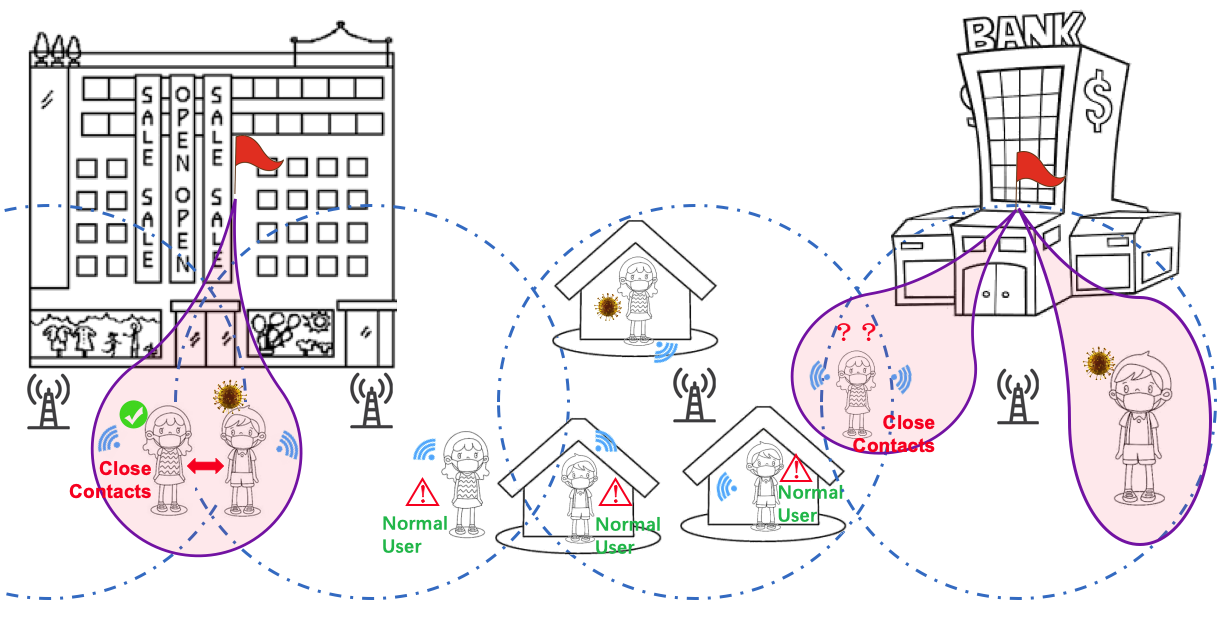
\includegraphics[width=0.45\textwidth]{figure/misclassification.png}
	\caption{Static Topology: The hollow circle in the network topology diagram represents a common terminal node, and the shaded positive pentagon represents the gateway. In this figure, the data is upward from left to right, and the distance between the node and the gateway is far and near. We sort the nodes on the same line parallel to the upstream direction into line 1, 2$\cdots$ and distinguish them by color.}\label{static}
\end{figure}


\subsection{Subsection Heading Here}
Subsection text here.


\subsubsection{Subsubsection Heading Here}
Subsubsection text here.


% An example of a floating figure using the graphicx package.
% Note that \label must occur AFTER (or within) \caption.
% For figures, \caption should occur after the \includegraphics.
% Note that IEEEtran v1.7 and later has special internal code that
% is designed to preserve the operation of \label within \caption
% even when the captionsoff option is in effect. However, because
% of issues like this, it may be the safest practice to put all your
% \label just after \caption rather than within \caption{}.
%
% Reminder: the "draftcls" or "draftclsnofoot", not "draft", class
% option should be used if it is desired that the figures are to be
% displayed while in draft mode.
%
%\begin{figure}[!t]
%\centering
%\includegraphics[width=2.5in]{myfigure}
% where an .eps filename suffix will be assumed under latex, 
% and a .pdf suffix will be assumed for pdflatex; or what has been declared
% via \DeclareGraphicsExtensions.
%\caption{Simulation results for the network.}
%\label{fig_sim}
%\end{figure}

% Note that the IEEE typically puts floats only at the top, even when this
% results in a large percentage of a column being occupied by floats.


% An example of a double column floating figure using two subfigures.
% (The subfig.sty package must be loaded for this to work.)
% The subfigure \label commands are set within each subfloat command,
% and the \label for the overall figure must come after \caption.
% \hfil is used as a separator to get equal spacing.
% Watch out that the combined width of all the subfigures on a 
% line do not exceed the text width or a line break will occur.
%
%\begin{figure*}[!t]
%\centering
%\subfloat[Case I]{\includegraphics[width=2.5in]{box}%
%\label{fig_first_case}}
%\hfil
%\subfloat[Case II]{\includegraphics[width=2.5in]{box}%
%\label{fig_second_case}}
%\caption{Simulation results for the network.}
%\label{fig_sim}
%\end{figure*}
%
% Note that often IEEE papers with subfigures do not employ subfigure
% captions (using the optional argument to \subfloat[]), but instead will
% reference/describe all of them (a), (b), etc., within the main caption.
% Be aware that for subfig.sty to generate the (a), (b), etc., subfigure
% labels, the optional argument to \subfloat must be present. If a
% subcaption is not desired, just leave its contents blank,
% e.g., \subfloat[].


% An example of a floating table. Note that, for IEEE style tables, the
% \caption command should come BEFORE the table and, given that table
% captions serve much like titles, are usually capitalized except for words
% such as a, an, and, as, at, but, by, for, in, nor, of, on, or, the, to
% and up, which are usually not capitalized unless they are the first or
% last word of the caption. Table text will default to \footnotesize as
% the IEEE normally uses this smaller font for tables.
% The \label must come after \caption as always.
%
%\begin{table}[!t]
%% increase table row spacing, adjust to taste
%\renewcommand{\arraystretch}{1.3}
% if using array.sty, it might be a good idea to tweak the value of
% \extrarowheight as needed to properly center the text within the cells
%\caption{An Example of a Table}
%\label{table_example}
%\centering
%% Some packages, such as MDW tools, offer better commands for making tables
%% than the plain LaTeX2e tabular which is used here.
%\begin{tabular}{|c||c|}
%\hline
%One & Two\\
%\hline
%Three & Four\\
%\hline
%\end{tabular}
%\end{table}


% Note that the IEEE does not put floats in the very first column
% - or typically anywhere on the first page for that matter. Also,
% in-text middle ("here") positioning is typically not used, but it
% is allowed and encouraged for Computer Society conferences (but
% not Computer Society journals). Most IEEE journals/conferences use
% top floats exclusively. 
% Note that, LaTeX2e, unlike IEEE journals/conferences, places
% footnotes above bottom floats. This can be corrected via the
% \fnbelowfloat command of the stfloats package.




\section{Conclusion}
The conclusion goes here.




% conference papers do not normally have an appendix


% use section* for acknowledgment
\section*{Acknowledgment}


The authors would like to thank...





% trigger a \newpage just before the given reference
% number - used to balance the columns on the last page
% adjust value as needed - may need to be readjusted if
% the document is modified later
%\IEEEtriggeratref{8}
% The "triggered" command can be changed if desired:
%\IEEEtriggercmd{\enlargethispage{-5in}}

% references section

% can use a bibliography generated by BibTeX as a .bbl file
% BibTeX documentation can be easily obtained at:
% http://mirror.ctan.org/biblio/bibtex/contrib/doc/
% The IEEEtran BibTeX style support page is at:
% http://www.michaelshell.org/tex/ieeetran/bibtex/
%\bibliographystyle{IEEEtran}
% argument is your BibTeX string definitions and bibliography database(s)
%\bibliography{IEEEabrv,../bib/paper}
%
% <OR> manually copy in the resultant .bbl file
% set second argument of \begin to the number of references
% (used to reserve space for the reference number labels box)
\begin{thebibliography}{1}

\bibitem{IEEEhowto:kopka}
H.~Kopka and P.~W. Daly, \emph{A Guide to \LaTeX}, 3rd~ed.\hskip 1em plus
  0.5em minus 0.4em\relax Harlow, England: Addison-Wesley, 1999.

\end{thebibliography}




% that's all folks
\end{document}


